\documentclass[letter]{article}
\usepackage{amsmath}
\usepackage{amsfonts}
\usepackage{amssymb}
\usepackage{ifthen}
\usepackage{fancyhdr}
\usepackage{graphicx}
\usepackage{subcaption}
\usepackage[shortlabels]{enumitem}

\newcommand{\fref}[1]{\textbf{Figure \ref{#1}}}

%%%
% Set up the margins to use a fairly large area of the page
%%%
\oddsidemargin=.2in
\evensidemargin=.2in
\textwidth=6in
\topmargin=0in
\textheight=9.0in
\parskip=.07in
\parindent=0in
\pagestyle{fancy}

%%%
% Set up the header
%%%
\newcommand{\setheader}[6]{
	\lhead{{\sc #1} {\sc #2}\\{} ({\small \it \today})}
	\rhead{
		{\bf #3} 
		\ifthenelse{\equal{#4}{}}{}{(#4)}\\
		{\bf #5} 
		\ifthenelse{\equal{#6}{}}{}{(#6)}%
	}
}

\begin{document}
	\setheader{CSC490}{Module 1}{Qiwen Hua}{}{Ben Weisz}{}
	
	\setcounter{section}{2}
	\subsection{LiDAR Voxelization}

	\textbf{Part 2:} In the implementation of the \verb|Voxelizer.forward| function, we map raw LiDAR points to voxels by taking the difference between the points and bounds (e.g. \verb|x_max|) and scale down by `step`. Therefore, larger \verb|step| yields lower resolution for the voxelized point clouds, thus decreasing the amount of captured information. 

	We can visualize the conclusion above by plotting the voxelized LiDAR point clouds for scene \verb|000| with four different \verb|step|s $\in \{0.25, 0.50, 1.00, 2.00\}$. The plots are shown below:

	\begin{figure}[h]
		\begin{subfigure}[t]{\textwidth}
			\centering
			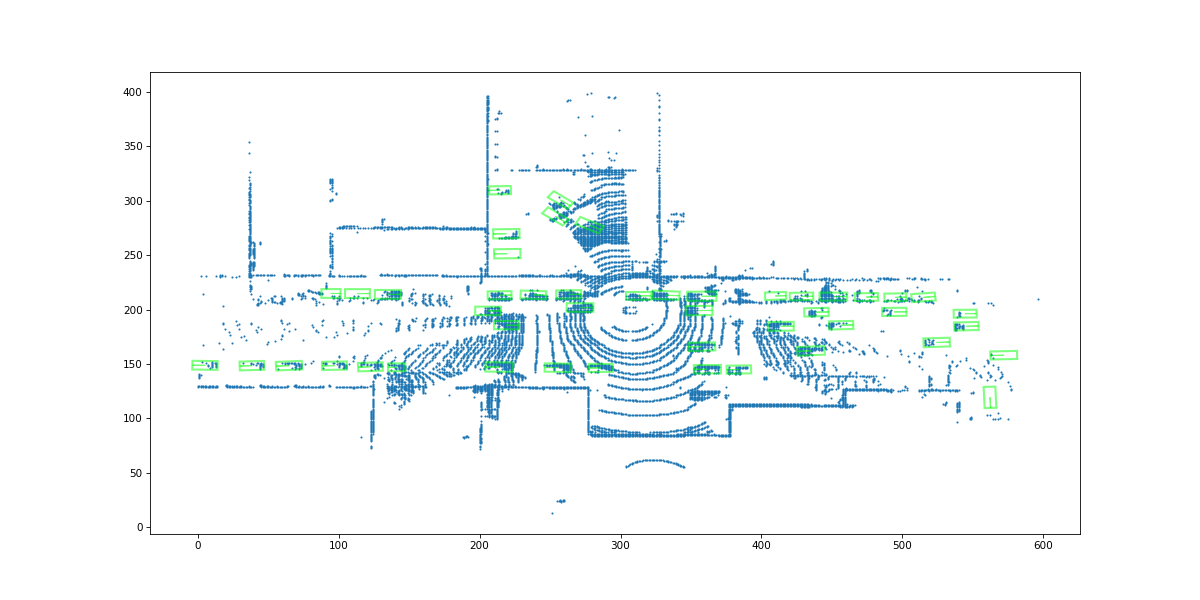
\includegraphics[width=\linewidth]{images/vox000_step0-25.png}
			\caption{step = 0.25}
		\end{subfigure}
		\vspace*{1mm}
	  
		\begin{subfigure}[t]{\textwidth}
			\centering
			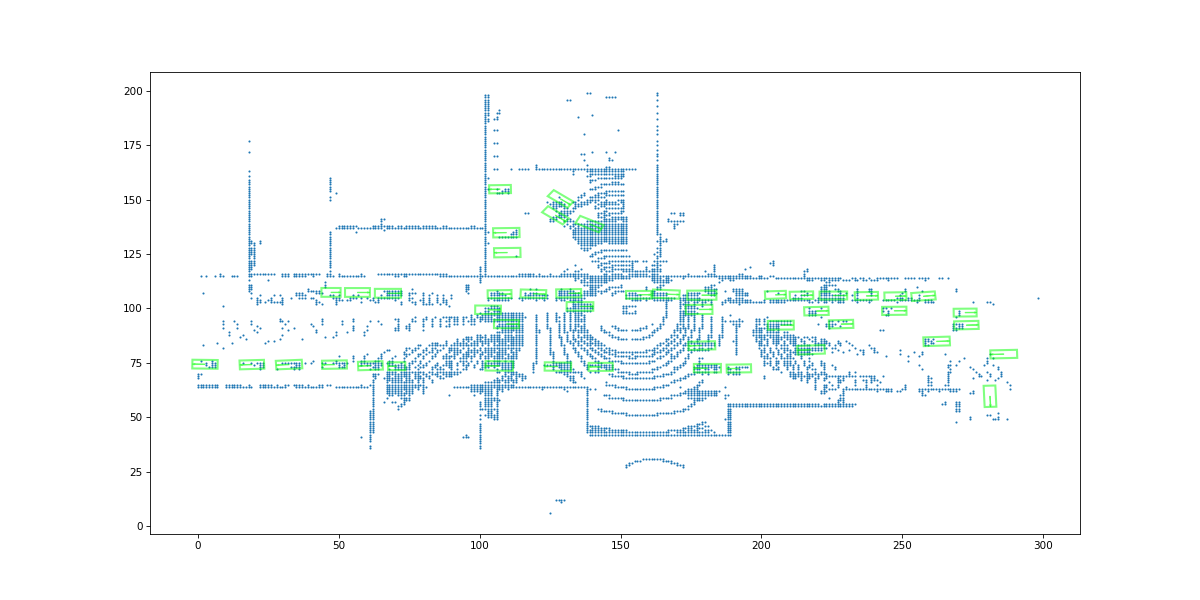
\includegraphics[width=\linewidth]{images/vox000_step0-50.png}
			\caption{step = 0.50}
		\end{subfigure}

		\caption{Voxelized LiDAR point clouds, part 1}
	\end{figure}

	\begin{figure}[h]
		\begin{subfigure}[t]{\textwidth}
			\centering
			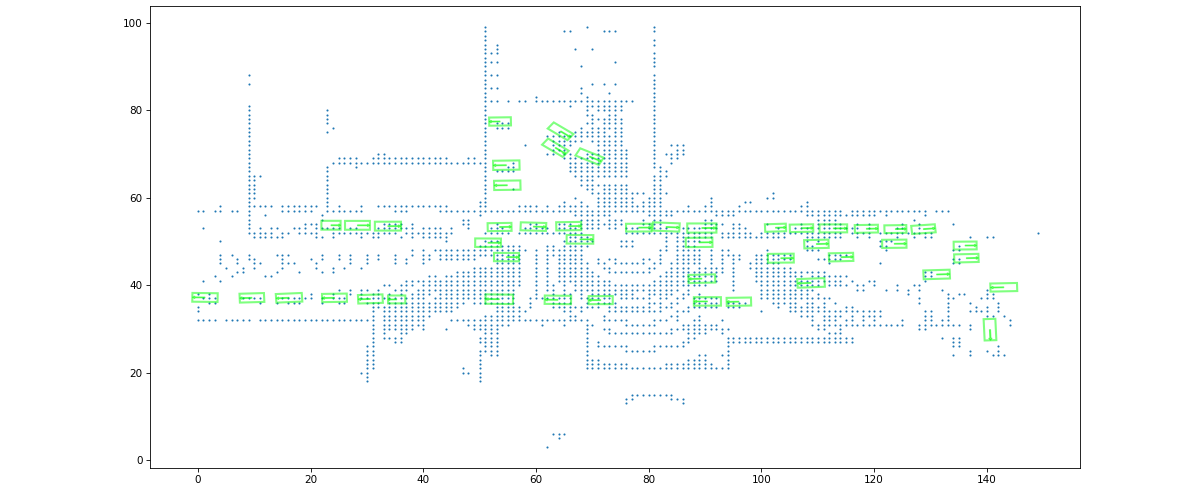
\includegraphics[width=\linewidth]{images/vox000_step1-00.png}
			\caption{step = 1.00}
		\end{subfigure}
		\vspace*{1mm}
	  
		\begin{subfigure}[t]{\textwidth}
			\centering
			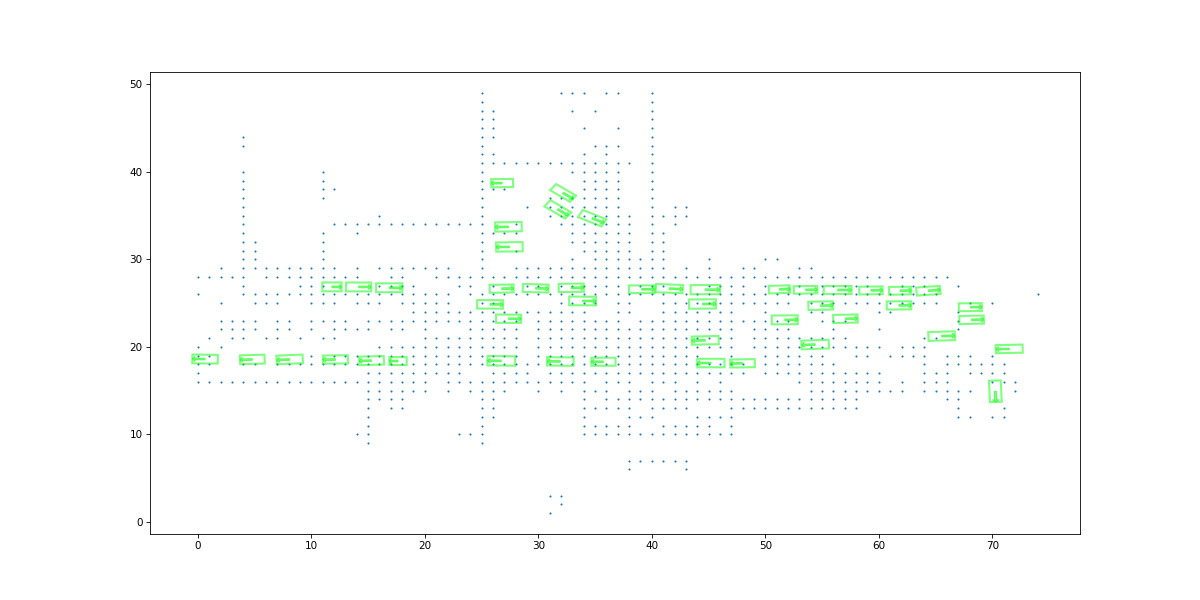
\includegraphics[width=\linewidth]{images/vox000_step2-00.png}
			\caption{step = 2.00}
		\end{subfigure}

		\caption{Voxelized LiDAR point clouds, part 2}
	\end{figure}

	From the plots above and below, we can see that the image with the highest resolution (Figure 1.a) captures much more information than the image with the lowest resolution (Figure 2.b). However, in order to have high fidelity of the voxel grid, the grid size also needs to be larger. Namely, image (Figure 1.a) has a size of 600 by 400 while image (Figure 2.b) has a size of 75 by 50; the size of the former grid is 64 times larger than the latter. 

	Therefore, we can conclude that the fidelity of the voxel grid comes at the cost of larger memory consumption (to store the larger grid). In addition, performance is also sacrificed as more captured information (voxel points) leading to more intensive computations. 

	\subsection{Model Training \& Inference}

	\textbf{Part 5:} We overfit the detector to a single frame of PandaSet using the \verb|overfit| command. The resulting detections after overfitting perfectly matches all labeled vehicles in centroids, sizes, and headings. 

	In the figure below (Figure 3), the green boxes represent the ground truth labels and the red boxes represent the detections:

	\begin{figure}[h]
		\centering
		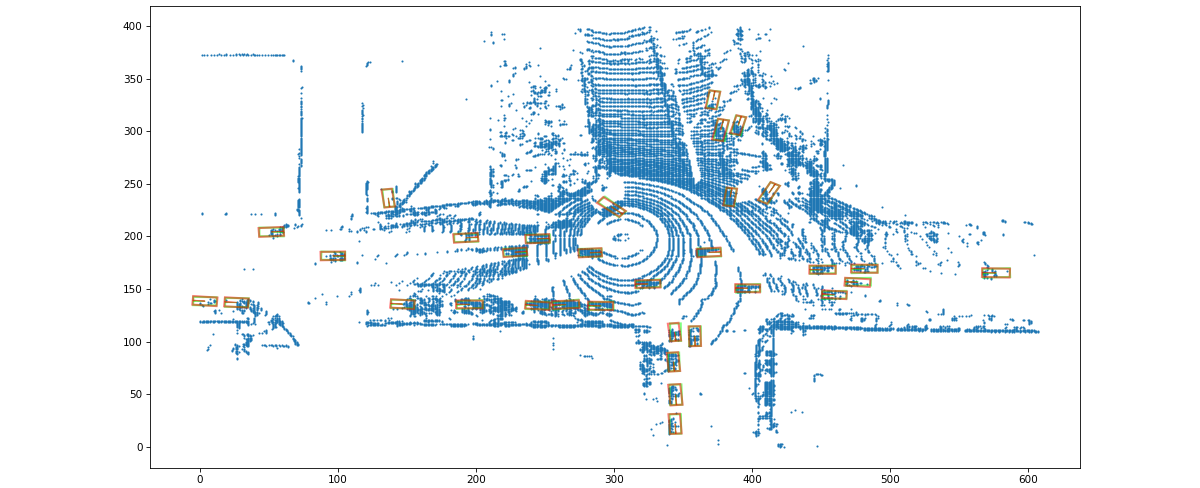
\includegraphics[width=\linewidth]{images/det_overfit.png}
		\caption{Detections after overfitting a single frame of PandaSet}
		\label{Label}
	\end{figure}

	\pagebreak
	\textbf{Part 6:} The original PandaSet dataset contains 47 sequences of LiDAR point clouds captured in intervals of 100ms. We first use 27 sequences to train the detector, then test the trained model on 12 different sequences for validation. Figure 4 below shows the detections of the model on four frames from the validation sequences.

	\begin{figure}[h]
		\begin{subfigure}[t]{0.49\textwidth}
			\centering
			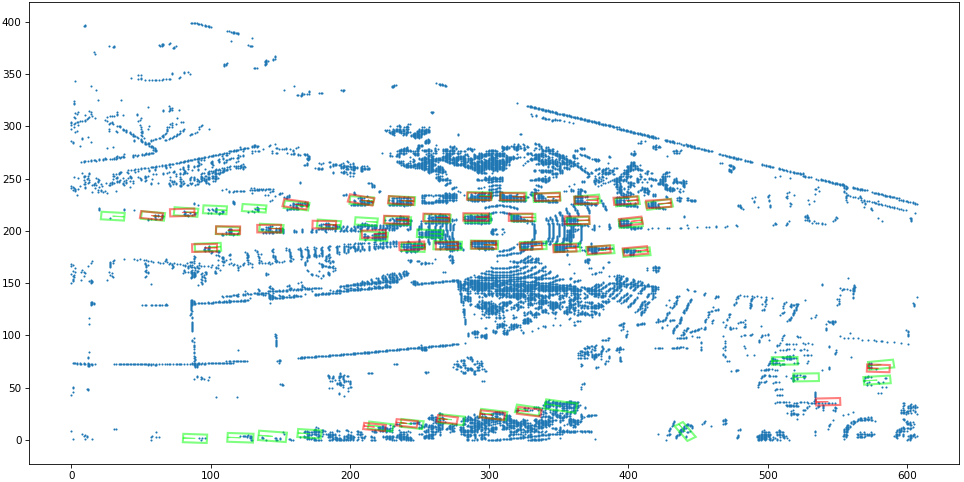
\includegraphics[width=\linewidth]{images/det_332.png}
			\caption{Detections for frame 332}
		\end{subfigure}
		\begin{subfigure}[t]{0.49\textwidth}
			\centering
			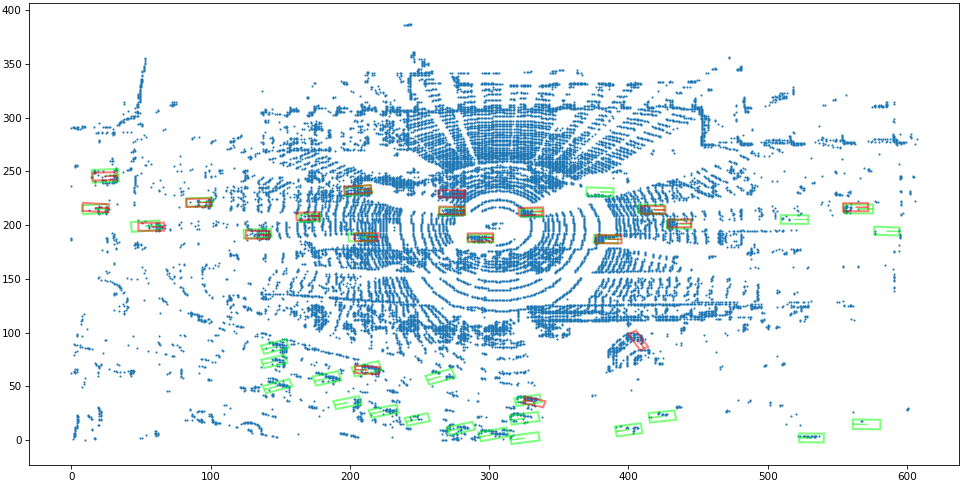
\includegraphics[width=\linewidth]{images/det_457.png}
			\caption{Detections for frame 457}
		\end{subfigure}
		\vspace*{1mm}
	  
		\begin{subfigure}[t]{0.49\textwidth}
			\centering
			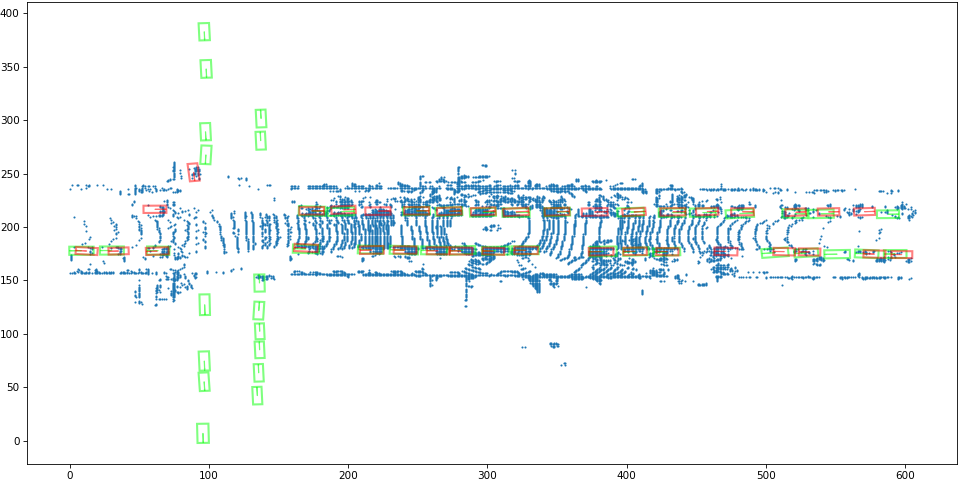
\includegraphics[width=\linewidth]{images/det_592.png}
			\caption{Detections for frame 592}
		\end{subfigure}
		\begin{subfigure}[t]{0.49\textwidth}
			\centering
			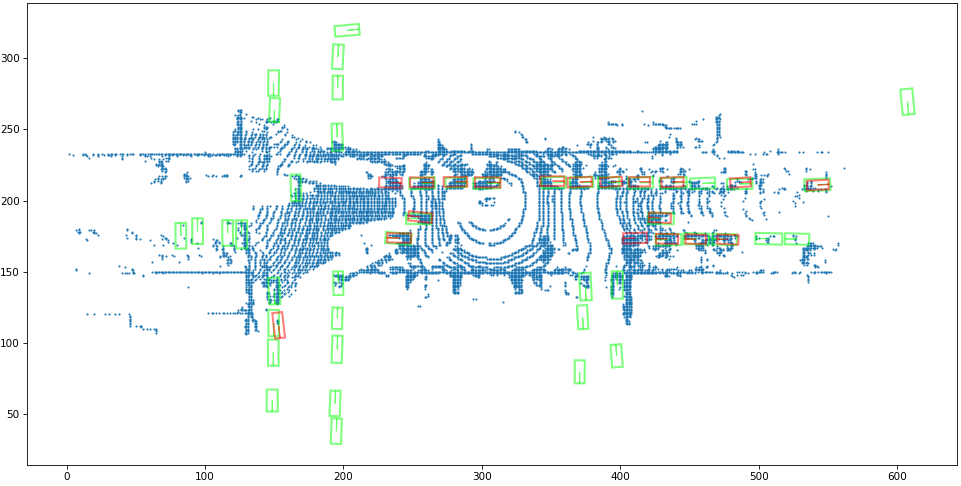
\includegraphics[width=\linewidth]{images/det_663.png}
			\caption{Detections for frame 663}
		\end{subfigure}

		\caption{Detections on frames from the validation sequences}
	\end{figure}

	From the four example frame detections above, we can see that the trained detector does a good job on detecting the centroids, sizes, and headings of the vehicles on the road, but performs poorly for vehicles off the road. This is likely due to the vehicles on the road are closer to the LiDAR sensors thus have more information captured in the LiDAR point clouds; note that some vehicles off the road do not have a single voxel in the grid. In addition, more vehicles would be detected if we adjust the activation heat threshold down, to allow the model to detect less confident vehicles. However, this would also increase the number of false positive detections. 

	\subsection{Evaluation}
	\setcounter{subsubsection}{2}
	\subsubsection{Average Precision \& PR Curve}
	Below we present the Precision-Recall curves for the values $2, 4, 8, 16$ of $\tau$.
	\begin{figure}[h]
		\centering
		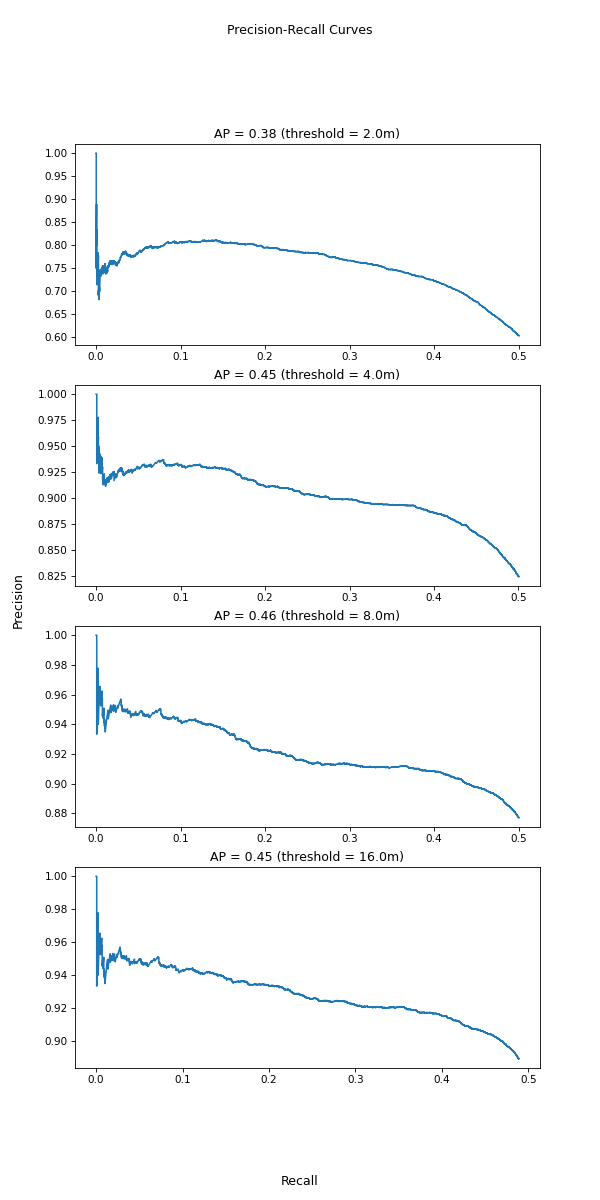
\includegraphics[scale=0.42]{images/prcurve.png}
		\caption{PR Curve for varying values for the distance threshold $\tau$}
		\label{fig:prcurve}
	\end{figure}
	\newpage
	The area under the curve of for $\tau=2.0, 4.0, 8.0, 16.0$ are presented in the following table.
	\begin{table}[!ht]
		\centering
		\begin{tabular}{|c|c|c|c|c|c|}
		\hline
		\textbf{Values of $\tau$} & 2.0 & 4.0 & 8.0 & 16.0 & \textbf{Mean} \\ \hline
		\textbf{Area Under Curve} & 0.3792 & 0.4521 & 0.4609 & 0.4539 & 0.4365177 \\ \hline
		\end{tabular}
		\caption{\label{tab:auc} AUC values for varying distace thresholds $\tau$}
	\end{table}

	When looking at \fref{fig:prcurve} we can see that as we increase our value of $\tau$ we start to see that the initial drop in precision for the top detections decreases. This means that for a larger value of $\tau$, We have less false positives among the top classified vehicles. This can be understood to be caused by how the false positive detections are considered. Since a larger range is considered, chances are that there is a label within the larger range for the value of $\tau$. As we increase $\tau$, we see that the overall precision also increases. Since $\tau$ is larger, the evaluation is much more free with which detections the labels may match.\\\\
	One possible method of getting a more accurate picture for the precision of the model would be to distinguish between which detection is paired with which label. This would give us a clearer picture for larger values of $\tau$ since the algorithm would be forced to pick one detection per label.\\\\
	The overall shape of the curves in \fref{fig:prcurve} match the expected shape for a precision-recall curve. For detections with lower detection scores we see that the false positive rate increases as the model is less and less sure about the correctness of the detections.\\\\
	In general, we see an overall increase in the average precision for the different values of $\tau$. Again, we can attribute this to the idea that for larger values of $\tau$ the matching algorithm is employed with less and less strictness of which detections match which labels.
	\subsubsection{Ground Truth}
	The ground truth for a given frame is computed by taking the data provide by the dataset and selecting for only those objects whose class is \verb|LabelClass.CAR|. Next we compute the centroid, the yaw, and the x and y sizes of the car. These values for the labels are computed as follows:\\\\
	\textbf{Centroids:}\\
	The centroid positions for cars are provided as 3D world positions in the original PandaSet. The first step is that the data loader converts these world based positions to positions relative to the self driving car. These are then provided as a label data to the another step which takes these vehicle space coordinates and projects out any out of bounds vehicle data from the frame. In addition to this the vehicle space positions are converted to image space so that the positions of the vehicles can be located in reference to the top left corner of the target image. This step is preformed by the voxelizer and it projects out the z coordinate of the vehicle space coordinates.\\\\
	\textbf{Yaw:}\\
	The yaw of the vehicles in a frame are provided relative to a forward direction. In order to provide the correct yaw with respect to the x and y axis of the desired target image, we must compensate for this relative rotation. The raw data specifies the yaw for the forward direction as a rotation matrix. The first step that the algorithm must take is to extract the yaw of the forward direction. With this yaw, and an additional offset constant of $\frac{\pi}{2}$, the yaw of the individual vehicle labels in the frame are compensated and the algorithm outputs the actual yaw with respect to the cardinal directions of the target image. Like for the centroid positions the yaws of the vehicles which are out of bounds are projected out.\\\\
	\newpage
	\textbf{Vehicle Sizes:}\\
	The dimensions of the vehicles in the PandaSet are first converted to from the right-up-forward to the left-front-up format. These dimensions are then passed to the voxelizer and are scaled by the voxelizers step size. This converts the vehicle dimensions from world space to the target image space units. Like with the other label parameters the voxelizer projects out the vehicle dimensions for those vehicles that are out of bounds for the given frame.\\\\
	Together the above three data points form the ground truth for the vehicles in the \verb|compute_average_precision| function. One way that the these transformations affect the data is that the labels which are out of bounds for the frame are removed. This leads to some loss of information for the system but this is a necessary sacrifice that must be made to lessen the computation needed to train the model. Additionally frame sizes need to be normalized to a constant size so that the number of model weights can be held constant. This leads the model to only learn information about vehicles within a certain distance of the self driving car.\\\\
	For regions of the transformed frame targets that have no point cloud data we cannot expect the the model to learn how to detect the labels in those regions. What is worse is that training on labels that have no surrounding point cloud data amounts training the network work to produce false positive detections. This phenomena can be seen in the top portion of the frame presented in \fref{fig:false-positive} with the green vehicle labels.
	
	\begin{figure}[h]
		\centering
		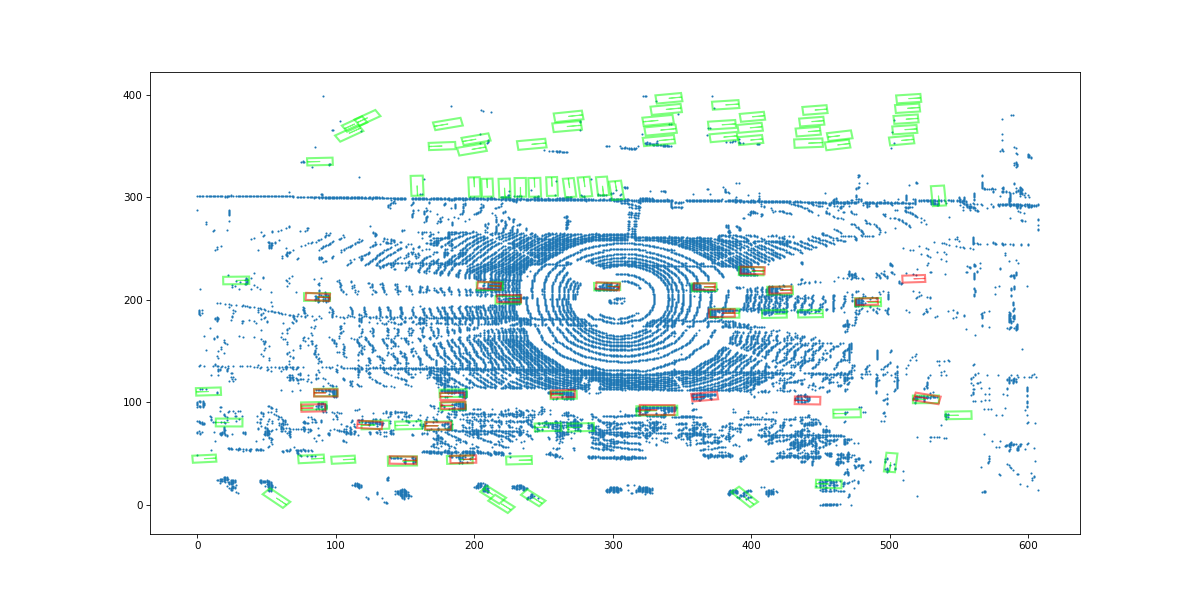
\includegraphics[width=\linewidth]{images/false-positives.png}
		\caption{Detection Frame showing false positives}
		\label{fig:false-positive}
	\end{figure}
	
\end{document}
